% Options for packages loaded elsewhere
\PassOptionsToPackage{unicode}{hyperref}
\PassOptionsToPackage{hyphens}{url}
\PassOptionsToPackage{dvipsnames,svgnames,x11names}{xcolor}
%
\documentclass[
  a4paper,
  DIV=11]{scrreprt}

\usepackage{amsmath,amssymb}
\usepackage{iftex}
\ifPDFTeX
  \usepackage[T1]{fontenc}
  \usepackage[utf8]{inputenc}
  \usepackage{textcomp} % provide euro and other symbols
\else % if luatex or xetex
  \usepackage{unicode-math}
  \defaultfontfeatures{Scale=MatchLowercase}
  \defaultfontfeatures[\rmfamily]{Ligatures=TeX,Scale=1}
\fi
\usepackage{lmodern}
\ifPDFTeX\else  
    % xetex/luatex font selection
\fi
% Use upquote if available, for straight quotes in verbatim environments
\IfFileExists{upquote.sty}{\usepackage{upquote}}{}
\IfFileExists{microtype.sty}{% use microtype if available
  \usepackage[]{microtype}
  \UseMicrotypeSet[protrusion]{basicmath} % disable protrusion for tt fonts
}{}
\makeatletter
\@ifundefined{KOMAClassName}{% if non-KOMA class
  \IfFileExists{parskip.sty}{%
    \usepackage{parskip}
  }{% else
    \setlength{\parindent}{0pt}
    \setlength{\parskip}{6pt plus 2pt minus 1pt}}
}{% if KOMA class
  \KOMAoptions{parskip=half}}
\makeatother
\usepackage{xcolor}
\setlength{\emergencystretch}{3em} % prevent overfull lines
\setcounter{secnumdepth}{5}
% Make \paragraph and \subparagraph free-standing
\ifx\paragraph\undefined\else
  \let\oldparagraph\paragraph
  \renewcommand{\paragraph}[1]{\oldparagraph{#1}\mbox{}}
\fi
\ifx\subparagraph\undefined\else
  \let\oldsubparagraph\subparagraph
  \renewcommand{\subparagraph}[1]{\oldsubparagraph{#1}\mbox{}}
\fi


\providecommand{\tightlist}{%
  \setlength{\itemsep}{0pt}\setlength{\parskip}{0pt}}\usepackage{longtable,booktabs,array}
\usepackage{calc} % for calculating minipage widths
% Correct order of tables after \paragraph or \subparagraph
\usepackage{etoolbox}
\makeatletter
\patchcmd\longtable{\par}{\if@noskipsec\mbox{}\fi\par}{}{}
\makeatother
% Allow footnotes in longtable head/foot
\IfFileExists{footnotehyper.sty}{\usepackage{footnotehyper}}{\usepackage{footnote}}
\makesavenoteenv{longtable}
\usepackage{graphicx}
\makeatletter
\def\maxwidth{\ifdim\Gin@nat@width>\linewidth\linewidth\else\Gin@nat@width\fi}
\def\maxheight{\ifdim\Gin@nat@height>\textheight\textheight\else\Gin@nat@height\fi}
\makeatother
% Scale images if necessary, so that they will not overflow the page
% margins by default, and it is still possible to overwrite the defaults
% using explicit options in \includegraphics[width, height, ...]{}
\setkeys{Gin}{width=\maxwidth,height=\maxheight,keepaspectratio}
% Set default figure placement to htbp
\makeatletter
\def\fps@figure{htbp}
\makeatother
% definitions for citeproc citations
\NewDocumentCommand\citeproctext{}{}
\NewDocumentCommand\citeproc{mm}{%
  \begingroup\def\citeproctext{#2}\cite{#1}\endgroup}
\makeatletter
 % allow citations to break across lines
 \let\@cite@ofmt\@firstofone
 % avoid brackets around text for \cite:
 \def\@biblabel#1{}
 \def\@cite#1#2{{#1\if@tempswa , #2\fi}}
\makeatother
\newlength{\cslhangindent}
\setlength{\cslhangindent}{1.5em}
\newlength{\csllabelwidth}
\setlength{\csllabelwidth}{3em}
\newenvironment{CSLReferences}[2] % #1 hanging-indent, #2 entry-spacing
 {\begin{list}{}{%
  \setlength{\itemindent}{0pt}
  \setlength{\leftmargin}{0pt}
  \setlength{\parsep}{0pt}
  % turn on hanging indent if param 1 is 1
  \ifodd #1
   \setlength{\leftmargin}{\cslhangindent}
   \setlength{\itemindent}{-1\cslhangindent}
  \fi
  % set entry spacing
  \setlength{\itemsep}{#2\baselineskip}}}
 {\end{list}}
\usepackage{calc}
\newcommand{\CSLBlock}[1]{\hfill\break\parbox[t]{\linewidth}{\strut\ignorespaces#1\strut}}
\newcommand{\CSLLeftMargin}[1]{\parbox[t]{\csllabelwidth}{\strut#1\strut}}
\newcommand{\CSLRightInline}[1]{\parbox[t]{\linewidth - \csllabelwidth}{\strut#1\strut}}
\newcommand{\CSLIndent}[1]{\hspace{\cslhangindent}#1}

\KOMAoption{captions}{tableheading}
\makeatletter
\@ifpackageloaded{tcolorbox}{}{\usepackage[skins,breakable]{tcolorbox}}
\@ifpackageloaded{fontawesome5}{}{\usepackage{fontawesome5}}
\definecolor{quarto-callout-color}{HTML}{909090}
\definecolor{quarto-callout-note-color}{HTML}{0758E5}
\definecolor{quarto-callout-important-color}{HTML}{CC1914}
\definecolor{quarto-callout-warning-color}{HTML}{EB9113}
\definecolor{quarto-callout-tip-color}{HTML}{00A047}
\definecolor{quarto-callout-caution-color}{HTML}{FC5300}
\definecolor{quarto-callout-color-frame}{HTML}{acacac}
\definecolor{quarto-callout-note-color-frame}{HTML}{4582ec}
\definecolor{quarto-callout-important-color-frame}{HTML}{d9534f}
\definecolor{quarto-callout-warning-color-frame}{HTML}{f0ad4e}
\definecolor{quarto-callout-tip-color-frame}{HTML}{02b875}
\definecolor{quarto-callout-caution-color-frame}{HTML}{fd7e14}
\makeatother
\makeatletter
\@ifpackageloaded{caption}{}{\usepackage{caption}}
\AtBeginDocument{%
\ifdefined\contentsname
  \renewcommand*\contentsname{Inhaltsverzeichnis}
\else
  \newcommand\contentsname{Inhaltsverzeichnis}
\fi
\ifdefined\listfigurename
  \renewcommand*\listfigurename{Abbildungsverzeichnis}
\else
  \newcommand\listfigurename{Abbildungsverzeichnis}
\fi
\ifdefined\listtablename
  \renewcommand*\listtablename{Tabellenverzeichnis}
\else
  \newcommand\listtablename{Tabellenverzeichnis}
\fi
\ifdefined\figurename
  \renewcommand*\figurename{Abbildung}
\else
  \newcommand\figurename{Abbildung}
\fi
\ifdefined\tablename
  \renewcommand*\tablename{Tabelle}
\else
  \newcommand\tablename{Tabelle}
\fi
}
\@ifpackageloaded{float}{}{\usepackage{float}}
\floatstyle{ruled}
\@ifundefined{c@chapter}{\newfloat{codelisting}{h}{lop}}{\newfloat{codelisting}{h}{lop}[chapter]}
\floatname{codelisting}{Listing}
\newcommand*\listoflistings{\listof{codelisting}{Listingverzeichnis}}
\makeatother
\makeatletter
\makeatother
\makeatletter
\@ifpackageloaded{caption}{}{\usepackage{caption}}
\@ifpackageloaded{subcaption}{}{\usepackage{subcaption}}
\makeatother
\ifLuaTeX
\usepackage[bidi=basic]{babel}
\else
\usepackage[bidi=default]{babel}
\fi
\babelprovide[main,import]{ngerman}
% get rid of language-specific shorthands (see #6817):
\let\LanguageShortHands\languageshorthands
\def\languageshorthands#1{}
\ifLuaTeX
  \usepackage{selnolig}  % disable illegal ligatures
\fi
\usepackage{bookmark}

\IfFileExists{xurl.sty}{\usepackage{xurl}}{} % add URL line breaks if available
\urlstyle{same} % disable monospaced font for URLs
\hypersetup{
  pdftitle={Statistik1},
  pdfauthor={Sebastian Sauer},
  pdflang={de},
  colorlinks=true,
  linkcolor={blue},
  filecolor={Maroon},
  citecolor={Blue},
  urlcolor={Blue},
  pdfcreator={LaTeX via pandoc}}

\title{Statistik1}
\author{Sebastian Sauer}
\date{2024-04-14}

\begin{document}
\maketitle

\renewcommand*\contentsname{Inhaltsverzeichnis}
{
\hypersetup{linkcolor=}
\setcounter{tocdepth}{2}
\tableofcontents
}
\chapter{Willkommen!}\label{willkommen}

\begin{figure}[H]

{\centering 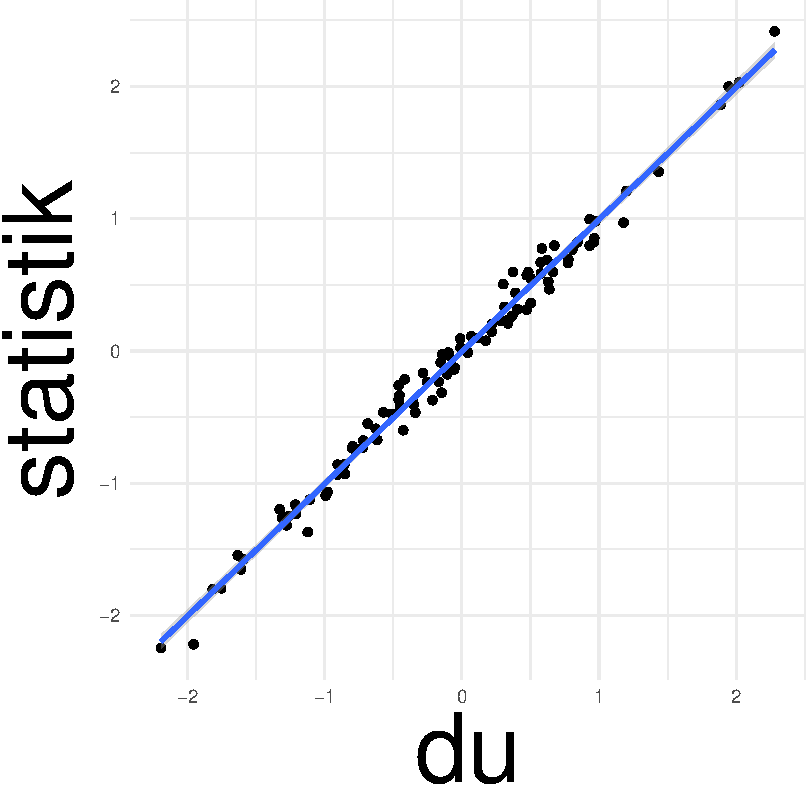
\includegraphics[width=0.33\textwidth,height=\textheight]{index_files/figure-pdf/unnamed-chunk-1-1.pdf}

}

\caption{Guter Fit}

\end{figure}%

Statistik und Du: Guter Fit!

\section{Es geht um Ihren Lernerfolg}\label{es-geht-um-ihren-lernerfolg}

Meister Yoda rät: Lesen Sie die Hinweise (Abbildung~\ref{fig-yoda}).

\begin{figure}

\centering{


\includegraphics[width=0.5\textwidth,height=\textheight]{img/yoda.jpg}

}

\caption{\label{fig-yoda}Lesen Sie die folgenden Hinweise im eigenen
Interesse}

\end{figure}%

\href{https://imgflip.com/memegenerator}{Quelle: Imgflip Memengenerator}

\subsection{Lernziele}\label{lernziele}

\begin{itemize}
\item
  Die Studentis sind mit wesentlichen Methoden der explorativen
  Datenanalyse vertraut und können diese selbständig anwenden.
\item
  Die Studentis können gängige Forschungsfragen in lineare Modelle
  übersetzen, diese auf echte Datensätze anwenden und die Ergebnisse
  interpretieren.
\end{itemize}

Kurz gesagt: Das ist ein Grundkurs in Daten zähmen.

\begin{figure}[H]

{\centering 
\includegraphics[width=0.5\textwidth,height=\textheight]{img/datenzaehmen.png}

}

\caption{Daten zähmen}

\end{figure}%

\href{https://github.com/allisonhorst/stats-illustrations}{Bildquelle:
Allison Horst, CC-BY}

\subsection{Was lerne ich hier und wozu ist das
gut?}\label{was-lerne-ich-hier-und-wozu-ist-das-gut}

\emph{Was lerne ich hier?}

Sie lernen das \emph{Handwerk der Datenanalyse} mit einem Schwerpunkt
auf Vorhersage. Anders gesagt: Sie lernen, \emph{Daten aufzubereiten}
und aus Daten \emph{Vorhersagen} abzuleiten. Zum Beispiel: Kommt ein
Student zu Ihnen und sagt ``Ich habe 42 Stunden für die Klausur gelernt,
welche Note kann ich in der Klausur erwarten?''. Darauf Ihre Antwort:
``Auf Basis meiner Daten und meines Modells müsstest du eine 2.7
schreiben!''.\footnote{Darauf dis Studenti: ``Hpmf.''}. Außerdem lernen
Sie, wie man die Güte einer Vorhersage auf Stichhaltigkeit prüft. Denn
Vorhersagen kann man ja in jeder Eckkneipe oder beim Wahrsager bekommen.
Wir wollen aber belastbare Vorhersagen und zumindest wissen, wie gut die
Vorhersagen (von jemanden) bisher waren.

\emph{Warum ist das wichtig?}

Wir wollen nicht auf Leuten vertrauen, die behaupten, sie wüssten, was
für uns richtig und gut ist. Wir wollen selber die Fakten prüfen können.

\emph{Wozu brauche ich das im Job?}

Datenanalyse spielt bereits heute in vielen Berufen eine Rolle. Tendenz
stark zunehmend.

\emph{Wozu brauche ich das im weiterem Studium?}

In Forschungsarbeiten (wie in empirischen Forschungsprojekten, etwa in
der Abschlussarbeit) ist es üblich, statistische Ergebnisse hinsichtlich
quantitativ zu analysieren.

\emph{Ist Statistik nicht sehr abstrakt?}

Der Schwerpunkt dieses Kurses liegt auf Anwenden und Tun; ähnlich dem
Erlernen eines Handwerks. Theorien und Abstraktionen stehen nur am Rand.

\emph{Gibt es auch gute Jobs, wenn man sich mit Daten auskennt?}

Das Forum (2020) berichtet zu den ``Top 20 job roles in increasing and
decreasing demand across industries'' (S. 30, Abb. 22):

\begin{enumerate}
\def\labelenumi{\arabic{enumi}.}
\tightlist
\item
  Data Analysts und Scientists
\item
  AI and Machine Learning Specialists
\item
  Big Data Specialists
\end{enumerate}

\subsection{Was ist hier das
Erfolgsgeheimnis?}\label{was-ist-hier-das-erfolgsgeheimnis}

\begin{tcolorbox}[enhanced jigsaw, toprule=.15mm, leftrule=.75mm, bottomrule=.15mm, opacitybacktitle=0.6, toptitle=1mm, coltitle=black, colback=white, rightrule=.15mm, left=2mm, colframe=quarto-callout-important-color-frame, breakable, title=\textcolor{quarto-callout-important-color}{\faExclamation}\hspace{0.5em}{Wichtig}, colbacktitle=quarto-callout-important-color!10!white, bottomtitle=1mm, titlerule=0mm, arc=.35mm, opacityback=0]

\emph{Dran bleiben} ist der Schlüssel zum Erfolg. \(\square\)

\end{tcolorbox}

\subsection{Motivieren Sie mich!}\label{motivieren-sie-mich}

Schauen Sie sich das Video mit einer
\href{https://youtu.be/jtNlzpcPr5Y}{Ansprache zur Motivation}
an.\footnote{\url{https://youtu.be/jtNlzpcPr5Y}}

\subsection{Voraussetzungen}\label{voraussetzungen}

Um von diesem Kurs am besten zu profitieren, sollten Sie Folgendes
mitbringen:

\begin{itemize}
\tightlist
\item
  Bereitschaft, Neues zu lernen
\item
  Bereitschaft, nicht gleich aufzugeben
\item
  Kenntnis grundlegender Methoden wissenschaftlichen Arbeitens
\end{itemize}

Was Sie \emph{nicht} brauchen, sind besondere Mathe-Vorkenntnisse.

\subsection{Überblick}\label{uxfcberblick}

Abb. Abbildung~\ref{fig-ueberblick} gibt einen Überblick über den
Verlauf und die Inhalte des Buches. Das Diagramm hilft Ihnen zu
verorten, wo welches Thema im Gesamtzusammenhang steht.

\begin{figure}

\centering{

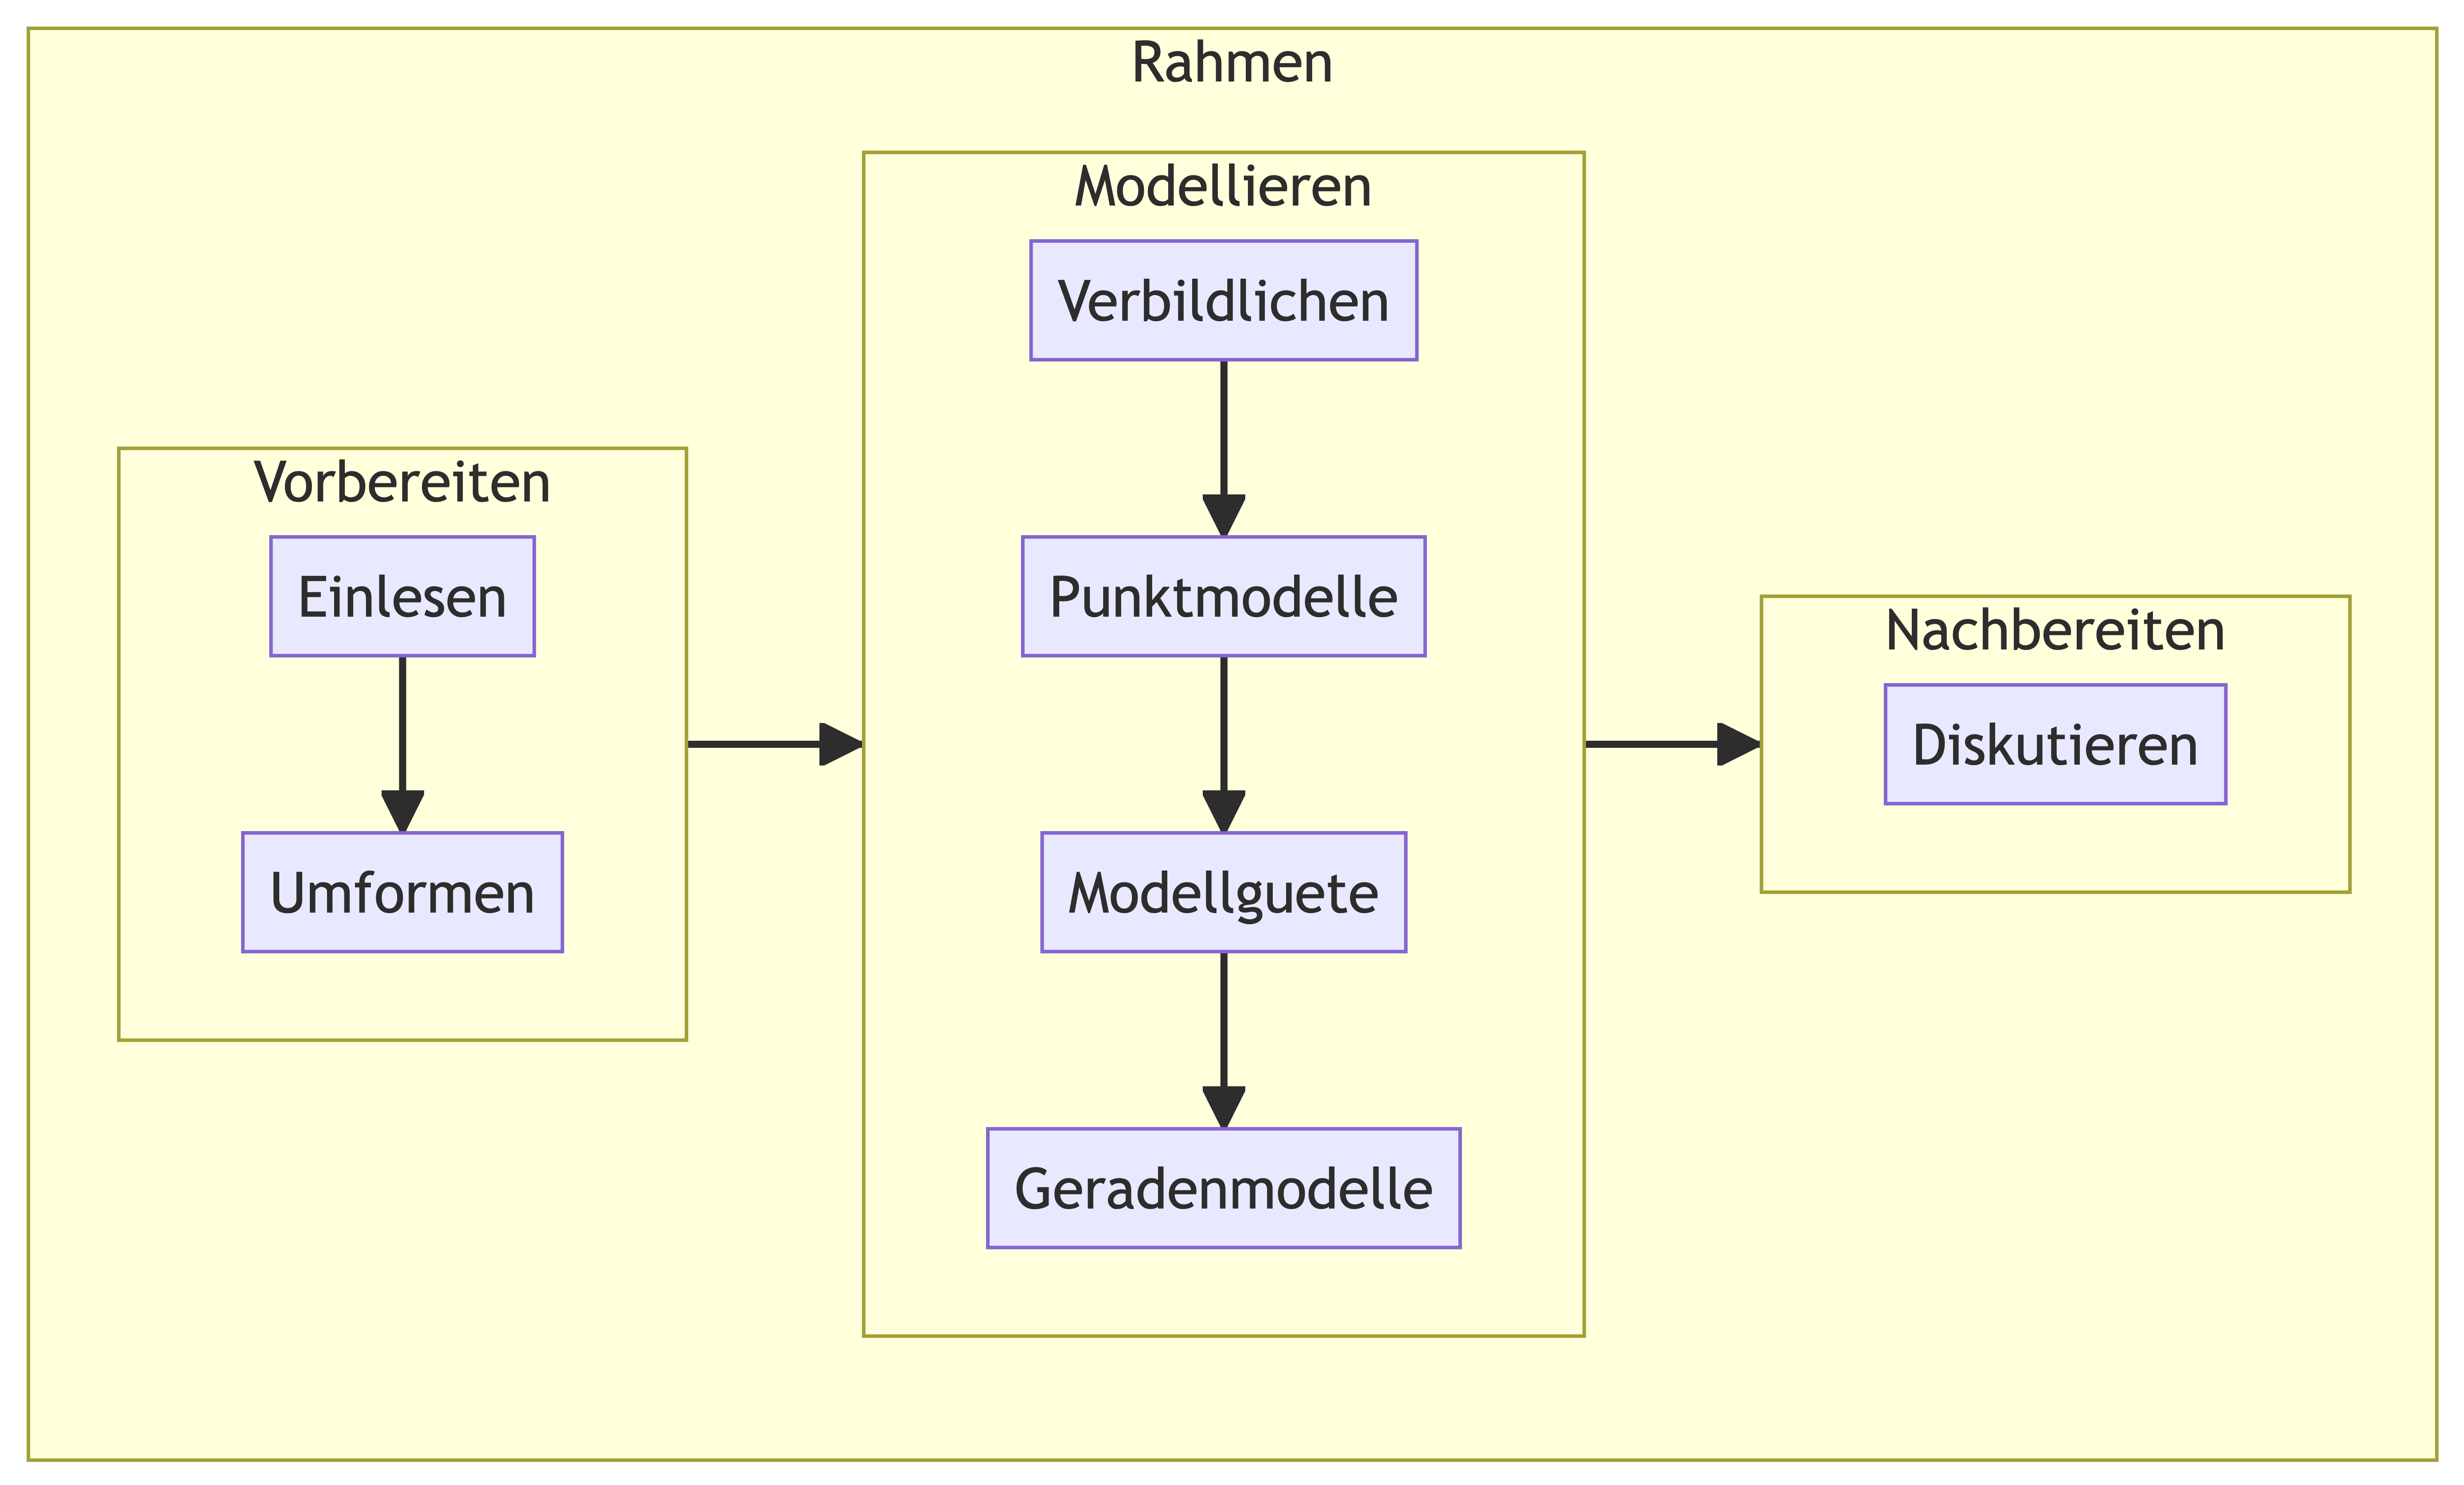
\includegraphics[width=7.24in,height=4.38in]{index_files/figure-latex/mermaid-figure-1.png}

}

\caption{\label{fig-ueberblick}Überblick über den Inhalt und Verlauf des
Buches}

\end{figure}%

Das Diagramm zeigt den Ablauf einer typischen Datenanalyse. Natürlich
kann man sich auch andere sinnvolle Darstellungen dieses Ablaufs
vorstellen.

\subsection{PDF-Version}\label{pdf-version}

Sie können die Druck-Funktion Ihres Broswers nutzen, um ein PDF-Dokument
eines Kapitels dieses Buchs zu erstellen.

\section{Software}\label{software}

Sie benötigen R, RStudio und einige R-Pakete für diesen Kurs.

\subsection{Installation}\label{installation}

\href{https://hinweisbuch.netlify.app/hinweise-software}{Hier} finden
Sie \emph{Installationshinweise.}\footnote{\url{https://hinweisbuch.netlify.app/hinweise-software}}

\subsection{Viel R (?)}\label{viel-r}

Dieses Buch enthält ``mittel'' viel R. Auf fortgeschrittene R-Techniken
wurde aber komplett verzichtet. Dem einen oder der anderen Anfänger:in
mag es dennoch ``viel Code'' erscheinen. Es wäre ja auch möglich
gewesen, auf R zu verzichten und stattdessen eine ``Klick-Software'' zu
verwenden. \href{https://jasp-stats.org/}{JASP} oder
\href{https://www.jamovi.org/}{Jamovi} sind Beispiele für tolle Software
aus dieser Kategorie. Ich glaube aber, der Verzicht auf eine
Skriptsprache (R) wäre ein schlechter Dienst an den Studentis. Mit Blick
auf eine ``High-Tech-Zukunft'' sollte man zumindest mit etwas
Computer-Code vertraut sein. Auf Computercode zu verzichten erschiene
mir daher fahrlässig für die ``Zukunftsfestigkeit'' der Ausbildung.

\section{Hinweise}\label{hinweise}

\begin{itemize}
\item
  📺
  \href{https://www.youtube.com/channel/UCkvdtj8maE7g-SOCh4aDB9g}{YouTube-Playlists
  zu Statistik}
\item
  \href{https://hinweisbuch.netlify.app/hinweise-lernhilfen-frame}{Lernhilfen}
\item
  \href{https://hinweisbuch.netlify.app/hinweise-didaktik-frame}{Didaktik}
\item
  \href{https://hinweisbuch.netlify.app/hinweise-unterricht-frame}{Unterrichtsorganisation}
\item
  Der Unterricht zu diesem Modul wird nur ein Mal pro Jahr angeboten
  (also nur jedes zweite Semester).
\item
  Eine Prüfung in diesem Modul ist jedes Semester möglich.
\end{itemize}

\section{Prüfung}\label{pruxfcfung}

\href{https://hinweisbuch.netlify.app/hinweise-pruefung-prognosewettbewerb-frame}{Im
Hinweisbuch} finden Sie Hinweise zur Prüfung.\footnote{\url{https://hinweisbuch.netlify.app/hinweise-pruefung-prognosewettbewerb-frame}}

\section{Zum Autor}\label{zum-autor}

Nähere Hinweise zum Autor dieses Buch, Sebastian Sauer, finden Sie
\href{https://sebastiansauer-academic.netlify.app/}{hier}.\footnote{\url{https://sebastiansauer-academic.netlify.app/}}
Dort gibt es auch einen Überblick über
\href{https://sebastiansauer-academic.netlify.app/\#ebooks}{weitere
Bücher des Autors zum Themenkreis Datenanalyse}.\footnote{\textless(https://sebastiansauer-academic.netlify.app/\#ebooks\textgreater{}}

\section{Nomenklatur}\label{nomenklatur}

\subsection{Griechische Buchstaben}\label{sec-greek}

In diesem Buch werden ein paar (wenige) griechische Buchstaben
verwendet, die in der Statistik üblich sind.

Häufig werden \emph{griechische} Buchstaben verwendet, um eine
Grundgesamtheit (Population) zu beschreiben (die meistens unbekannt
ist). Lateinische (``normale'') Buchstaben werden demgegenüber
verwendet, um eine Stichprobe (Datensatz, vorliegende Daten) zu
beschreiben.

Tabelle~\ref{tbl-griech} stellt diese Buchstaben zusammen mit ihrer
Aussprache und Bedeutung vor.

\begin{longtable}[]{@{}lllr@{}}
\caption{Griechische Buchstaben, die in diesem Buch verwendet
werden.}\label{tbl-griech}\tabularnewline
\toprule\noalign{}
Zeichen & Aussprache & Buchstabe & Bedeutung in der Statistik \\
\midrule\noalign{}
\endfirsthead
\toprule\noalign{}
Zeichen & Aussprache & Buchstabe & Bedeutung in der Statistik \\
\midrule\noalign{}
\endhead
\bottomrule\noalign{}
\endlastfoot
\(\beta\) & beta & b & Regressionskoeffizent \\
\(\mu\) & mü & m & Mittelwert \\
\(\sigma\) & sigma & s & Streuung \\
\(\Sigma\) & Sigma & S & Summenzeichen \\
\(\rho\) & rho & r & Korrelation (nach Pearson) \\
\end{longtable}

Mehr griechische Buchstaben finden sich
\href{https://de.wikipedia.org/wiki/Griechisches_Alphabet}{z.B. in
Wikipedia}.

\section{Zitation}\label{zitation}

Bitte zitieren Sie dieses Buch wie folgt:

\begin{quote}
Sauer, S. (2024). \emph{Statistik1}. https://statistik1.netlify.app/
\end{quote}

Hier sind die maschinenlesbaren Zitationsinfos (Bibtex-Format), die Sie
in Ihre Literatursoftware importieren können:

\begin{verbatim}
@book{sauer_statistik1,
    title = {Statistik1},
    rights = {CC-BY-NC},
    url = {https://statistik1.netlify.app/},
    author = {Sauer, Sebastian},
    date = {2024},
}
\end{verbatim}

Hier ist die DOI:

\href{https://zenodo.org/doi/10.5281/zenodo.10082517}{10.5281/zenodo.10082517}

\section{Reproduzierbarkeit}\label{reproduzierbarkeit}

Die verwendeten R-Pakete sind mit
\href{https://rstudio.github.io/renv/index.html}{renv}
dokumentiert.\footnote{\url{https://rstudio.github.io/renv/index.html}}

Der Quellcode ist \href{https://github.com/sebastiansauer/statistik1}{in
diesem Github-Repo} dokumentiert.\footnote{\url{https://github.com/sebastiansauer/statistik1}}

Dieses Dokument wurde erzeugt am/um 2024-04-07 17:58:12.

\section{Literatur}\label{literatur}

\part{Organisatorisches}

\phantomsection\label{refs}
\begin{CSLReferences}{1}{0}
\bibitem[\citeproctext]{ref-world_economic_forum_future_2020}
Forum, W. E. (2020). \emph{The {Future} of {Jobs Report} 2020}. World
Economic Forum.
\url{https://www3.weforum.org/docs/WEF_Future_of_Jobs_2020.pdf}

\end{CSLReferences}



\end{document}
